\documentclass[main.tex]{subfiles}
\begin{document}

\section{Lorem}

\begin{frame}{Highlight}
	\begin{center}
		\Large
		online immer lieber {\Huge mehr} als weniger\\
		und häufig wechseln!
	\end{center}
	\pause
	\begin{center}
		\Large
		Das bringt Abwechslung und Bewegung\\auf
		den Bildschirm und hilft,\\
		{\Huge Aufmerksamkeit} zu {\Huge halten}.
	\end{center}
\end{frame}

\begin{frame}{Kolom gambar dan teks}
	\begin{columns}
		\begin{column}{5cm}
			\begin{center}
				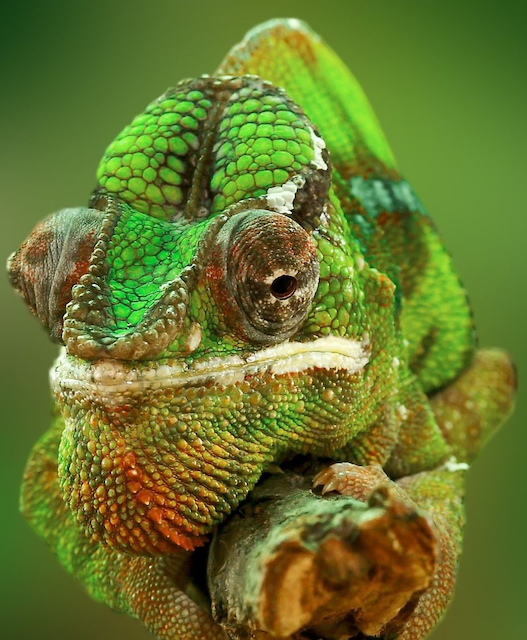
\includegraphics[height=6cm]{figures/chamaeleon_hochformat}

				{\tiny \textcolor{digiPH_darkorange}{Bildquelle: \url{pixabay.com}, CC-0}}
			\end{center}
		\end{column}
		\begin{column}{5cm}
			\begin{center}
				\Large
				Bitte mit Bedacht!
			\end{center}
			\pause
			\begin{center}
				Nicht mehr als ein bis zwei verschiedene Schriftfarben verwenden (Ruhe, bessere Lesbarkeit).
			\end{center}
			\begin{center}
				Tipp: Lieber durch Bilder Abwechslung schaffen!
			\end{center}
		\end{column}
	\end{columns}
\end{frame}

\begin{frame}
	%Gambar besar dengan penjelasan tanpa judul
	\begin{center}
		
\includegraphics[height=6cm]{figures/kopfhoerer}

		{\tiny \textcolor{digiPH_darkorange}{Nicht die Bildquelle und die Lizenz vergessen! Bildquelle: \url{pixabay.com}, CC-0}}
	\end{center}
	\begin{center}
		Haben Sie Mut zur Vereinfachung und zu ungewohnter Positionierung und finden Sie interessante Ausschnitte.
	\end{center}
\end{frame}

\begin{frame}{Gambar besar dengan judul dan penjelasan}
	\begin{center}
		
\includegraphics[height=5.5cm]{figures/placeholder}

		{\tiny \textcolor{digiPH_darkorange}{Bildquelle: \url{pixabay.com}, CC-0}}
	\end{center}
	\begin{center}
		Geschlechtsneutrales Formulieren ist uns wichtig: bei unseren eLectures ebenso. \textbf{In Schrift, Wort und Bild!}
	\end{center}
\end{frame}


\begin{frame}{Gambar dengan penjelasan sebelumnya}
	\small Ihre eLecture wird zum Nachsehen aufgezeichnet und veröffentlicht. Deshalb muss sie inhaltlich und urheberrechtlich korrekt sein!

	\tiny Weiteres dazu entnehmen Sie bitte dem Infoblatt: \url{http://www.virtuelle-ph.at/selbst-electures-abhalten/infoblatt}

	\small Die Teilnehmenden werden über einen Disclaimer zu Beginn der eLecture darüber informiert:

	\begin{center}
		
\includegraphics[height=3.5cm]{figures/placeholder}

		{\tiny \textcolor{digiPH_darkorange}{Bildquelle: Lene Kieberl, \href{https://creativecommons.org/licenses/by/3.0/at/}{CC BY}}}
	\end{center}
\end{frame}

\begin{frame}[t]{Tiga Gambar}

	\hfil\hfil
\includegraphics[width=5cm]{figures/placeholder}\newline
	\null\hfil\hfil\makebox[5cm]{Lorem}\newline
	\vfil
	\hfil\hfil{
\includegraphics[width=5cm]{figures/placeholder}}\hfil\hfil
	{
\includegraphics[width=5cm]{figures/placeholder}}\newline
	\null\hfil\hfil{\makebox[5cm]{Lorem}}
	\hfil\hfil{\makebox[5cm]{Lorem}}

\end{frame}

\begin{frame}{Kolom dengan foto orang}
	\begin{columns}
		\begin{column}{5cm}
			\small besonders aber bei Minderjährigen bitte unbedingt abklären, ob diese bzw. ihre Erziehungsberechtigten mit der Veröffentlichung einverstanden sind (Recht am eigenen Bild).
		\end{column}
		\begin{column}{5cm}
			\begin{center}
				
\includegraphics[height=2.5cm]{figures/placeholder}

				{\tiny \textcolor{digiPH_darkorange}{Bildquelle: Details Foto XY, \url{pixabay.com}, CC-0}}
			\end{center}
		\end{column}
	\end{columns}
	\begin{columns}
		\begin{column}{5cm}
			\begin{center}
				
\includegraphics[width=5cm]{figures/placeholder}

				{\tiny \textcolor{digiPH_darkorange}{Bildquelle: Details Foto XY, \url{pixabay.com}, CC-0}}
			\end{center}
		\end{column}
		\begin{column}{5cm}
			\begin{block}{\small Tipp:}
				\scriptsize
				Als Hilfestellung können Sie vielleicht unseren \enquote{Schummelzettel OER} mit Tipps und Quellen für verwendbare Bilder nutzen, den Sie hier zum Download vorfinden:\\
				\url{http://www.virtuelle-ph.at/schummelzettel}
			\end{block}
		\end{column}
	\end{columns}
\end{frame}

\begin{frame}{Sie möchten Software/Seiten live vorzeigen?}
	% Schriftgröße verkleinern
	\scriptsize
	% Absatzabstand einstellen
	\setlength{\parskip}{0.75\baselineskip}

	Beachten Sie bitte, dass Sie beim Zeigen von längeren Ausschnitten einer \textbf{Programmoberfläche} (Vorzeigen von Abläufen die nicht mehr durch das Zitatrecht abgedeckt sind) gegebenenfalls die \textbf{Erlaubnis der Herstellerfirma einholen müssen}, sofern Sie nicht Urheber/in sind bzw. keine lizenzrechtliche Erlaubnis zur Vorführung vorliegt (mehr Info: \url{http://bit.ly/vphuhr}).

	\textbf{Diese Angabe kann Ihre Co-Moderation für Sie einblenden, bitte teilen Sie sie bei Testtermin oder via Email mit.}

	\begin{block}{\scriptsize Beispiel: Live-Demo \href{GIMP}{http://www.gimp.org/},GNU General Public License 29.01.2018}
		\centering
		
\includegraphics[height=4cm]{figures/placeholder}
	\end{block}
\end{frame}


% Hanya untuk Navigasi Miniframe
\miniframesoff
\begin{frame}<beamer>{}
	\begin{center}
		\ldots Manege frei für Ihr Knowhow und Ihre Folien!
	\end{center}
	\vspace{3cm}
	\tiny
	PS: Am Ende Ihrer eLecture weist Ihre Co-Moderation die Teilnehmenden noch auf weitere Angebote (\zB der aktuellen Online-Tagung) und die Social-Media-Präsenzen hin. Wir bitten Sie auch um Weiterverbreitung unseres (und Ihres!) Lernangebots. Selbst schon geliked? Wir freuen uns über Likes, Kommentare und natürlich Follower!
\end{frame}

%\begin{frame}{\enquote{Stopfen} Gambar dengan qoute digambar \ldots}
%   \framesubtitle{Arbeiten Sie mit Bildern: online lieber mehrere, weniger dichte Folien zeigen!}
%   \begin{center}
%       \begin{tikzpicture}
%           \node[anchor=south west,inner sep=0] (bild) at (0,0) {
\includegraphics[width=0.88\textwidth]{figures/placeholder}};
%           \begin{scope}[x=(bild.south east),y=(bild.north west)]
%               % Gitternetz einzeichnen
%               %\draw[help lines] (0,0) grid[xstep=0.1,ystep=0.1] (1,1);
%               % Text einfügen
%               \node[font=\scriptsize,align=left,color=white,text width=4cm] (text) at (0.79,0.3) {Bitte verwenden Sie ausschließlich urheberrechts-einwandfreies Bildmaterial (NoGo: Schulbücher!)\\
%               Am besten also: eigenes und/oder CC-Bildmaterial, \zB von \url{www.pixabay.com} oder ähnlichen Plattformen!\\
%               Bitte nie eine sichtbare Bildquelle und Lizenz vergessen.};
%           \end{scope}
%       \end{tikzpicture}
%
%       {\tiny \textcolor{digiPH_darkorange}{Bildquelle: David Bogner, 2015, \href{https://creativecommons.org/licenses/by-nc-sa/3.0/at/}{CC BY-NC-SA}}}
%   \end{center}
%\end{frame}

\end{document}
